In this project there needs to be data to transmit,The network needs to be able to:
\begin{enumerate}
	\item Transmit  data for  example  temperature, humidity,light and camera images.
	\item Read data every hour  and  stored it as a CSV file, The image file  will depend on the module chosen
	\item Detect  any animal that passes  the  node with a motion sensor. 
\end{enumerate}
\newpage
The following is  a  rough circuit diagram  for the project:
\begin{figure}[h!]
	\centering
	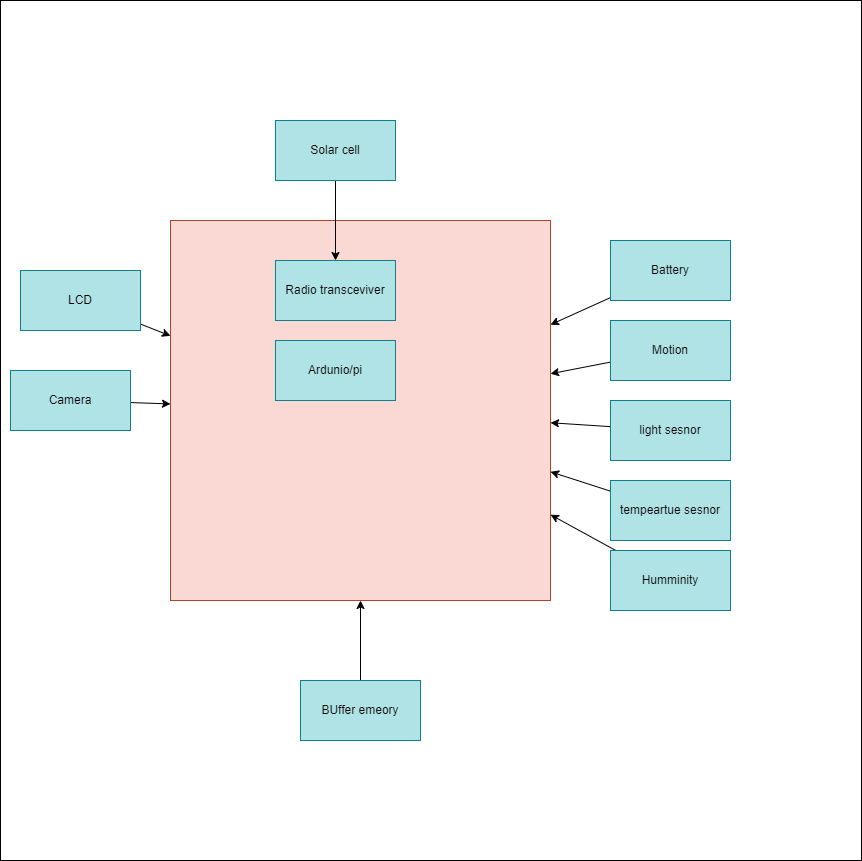
\includegraphics[width=0.5\linewidth]{Images/block_diagram_for_mesh_device.png}
	\caption{Rough circuit diagram for project}
	\label{Rough circuit diagram for project}
\end{figure}
\begin{enumerate}
	\item A PCB cannot be used due to  the ordering process taking too long for the time frame of this project 
	\item Any  type of board like wire wrap  would take too long and would be outside of  the  goals of this project
	\item A  choice of either the  Arduino or Raspberry Pi is left
\end{enumerate}
This section discusses the following:
\begin{enumerate}
	\item The sensors to be used in the project
	\item The ADC we will have  to will have to  consider
	\item The camera chosen will have to be  considered  for this project
	\item The memory module considerations
	\item The battery chosen
	\item A choice made between Arduino or Raspberry PI
\end{enumerate}

\subsection{Sensor considerations}
In this section, the process of  considering each component of the sensors will be discussed.
These components are:
\begin{enumerate}
	\item Temperature
	\item Humidity
	\item Light
	\item Motion
\end{enumerate}
\subsubsection{Temperature \& Humidity sensor}
The sensor needs to be able to work in the following conditions:
\begin{enumerate}
	\item The mesh node will be outside
	\item The device is in Ireland		\item The device is in a forest
\end{enumerate}
Taking these requirements into consideration,the temperature in Ireland was researched.

The following table was obtained from Met Eireann \cite{Eirrean}. which shows  the highest air temperature in a  shaded area
\begin{table}[h!]
	\begin{tabular}{ | c | c | c | }
		\hline
		Highest Shaded Air (°C) & Station & Date \\ \hline
		18.5°C & Dublin (Glasnevin) & 10th 1998 \\ \hline
		18.1°C & Dublin (Phoenix Park) & 23rd 1891 \\ \hline
		23.6°C & Dublin (Trinity College) & 28th 1965 \\ \hline
		25.8°C & Donegal (Glenties) & 26th 1984 \\ \hline
		28.4°C & Kerry (Ardfert Liscahane) & 31st 1997 \\ \hline
		33.3°C & Kilkenny (Kilkenny Castle) & 26th 1887 \\ \hline
		33.0°C & Dublin (Phoenix Park) & 18th 2022 \\ \hline
		31.7°C & Carlow (Oak Park) & 12th 2022 \\ \hline
		29.1°C & Kildare (Clongowes Wood College) & 1st 1906 \\ \hline
		25.2°C & Kildare (Clongowes Wood College) & 3rd 1908 \\ \hline
		20.1°C & Kerry (Dooks) & 1st 2015 \\ \hline
		18.1°C & Dublin (Peamount) & 2nd 1948 \\ \hline
		\end{tabular}
		\caption{Highest shader air Met Eireann(13$^{th}$ June 2023)}
		\label{Highest shader air Met eirrean}
	\end{table}

According to the table, the highest temperature is 33.3.The  other  extreme of the Lowest temperature was then considered:
	\begin{table}[h!]
		\begin{tabular}{ | c | c | c | }
		\hline
		Lowest Shaded Air (°C) & Station & Date \\ \hline
		-19.1°C & Sligo (Markree) & 16th 1881 \\ \hline
		-17.8°C & Longford (Mostrim) & 7th 1895 \\ \hline
		-17.2°C & Sligo (Markree) & 3rd 1947 \\ \hline
		-7.7°C & Sligo (Markree) & 15th 1892 \\ \hline
		-5.6°C & Donegal (Glenties) & 4th 1979 \\ \hline
		-3.3°C & Offaly (Clonsast) & 1st 1962 \\ \hline
		-0.3°C & Longford (Mostrim) & 8th 1889 \\ \hline
		-2.7°C & Wicklow (Rathdrum) & 30th 1964 \\ \hline
		-3.5°C & Offaly (Clonsast) & 8th 1972 \\ \hline
		-8.3°C & Sligo (Markree) & 31st 1926 \\ \hline
		-11.5°C & Wexford (Clonroche) & 29th 2010 \\ \hline
		-17.5°C & Mayo (Straide) & 25th 2010 \\ \hline
		\end{tabular}
	\caption{Lowest shader air Met Eireann(13$^{th}$ June 2023)}
	\label{Lowest shader air Met eirrean}	
	\end{table}

According to the table above the lowest temp is -19.1
In consideration for where the project the condition is a range of -19.1\textdegree C to 33.3\textdegree C.
\newpage
Humdity was also researched,Humidity refers to the amount of water vapeor in the air. The following table was obtained from Met Eireann \cite{eirrean2}:
\begin{table}[h!]
	\begin{tabular}{|c|c|c|c|c|c|c|c|c|c|c|c|c|c|}
		\hline
		\space & Jan & Feb & Mar & Apr & May & Jun & Jul & Aug & Sep & Oct & Nov & Dec & Year \\
		\hline
		Mean at 0900UTC &87.0 &86.4&84.0&79.5&76.9&76.7&78.5&81.0&83.4&85.5&88.5&88.0&83.0 \\
		Mean at 1500UTC &80.6&75.7&71.0&68.3&68.0&68.3&69.0&69.3&71.5&75.1&80.3&83.1&73.3\\
		\hline
	\end{tabular}
	\caption{Realtive Humidity(\%) according to met eirrean}
	\label{Realtive Humidity according to met eirrean}
\end{table}

The ranges are from 68.3\% to 88 \% Taking these considerations into account.Here are the different components:

\begin{table}[h!]
	\centering
	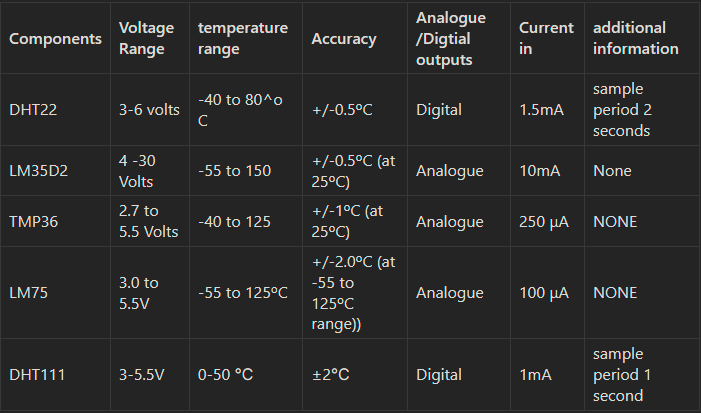
\includegraphics[width=0.5\linewidth]{Images/tempssenorscompared.png}
	\caption{Comparing of temperature sensors}
	\label{Comparing of temperature sensors}
\end{table}
After this, the choice between two sensors was narrowed down to DHT22 and DHT11. The  following are the advantages and disadvantages of the DHT22 and DHT11:
\begin{table}[h!]
	\centering
	\scalebox{0.8}{\begin{tabular}{|c|c|c|}
	\hline
		Device & Advantages & Disadvantages  \\
		\hline
		\hline
		DHT22 & good accuracy has temp and humidity, falls in our temp range & sample period 2 seconds \\
		\hline
		DHT11 & OK voltage,better sample period & draws a lot of current , and our of range \\
	\hline
	\end{tabular}}
	\caption{Comparing DHT22 and DHT11}
	\label{Compareing DHT22 and DHT11}

\end{table}

 DHT22 was chosen. Which has a  Digital output. See a wiring diagram next page:
 \newpage
This will have an interface of the following:

\begin{figure}[h!]
	\centering
	\begin{subfigure}{0.6\textwidth}
		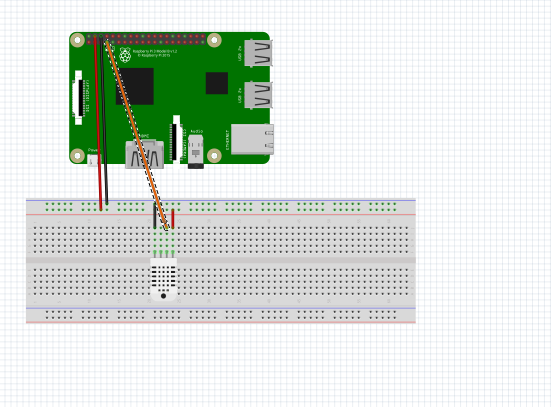
\includegraphics[width=\textwidth]{Images/InterfaceforDHT22.png}
		\caption{Interface for DHT22}
		\label{Interface for DHT22}
	\end{subfigure}
	\hfill
	\begin{subfigure}{0.6\textwidth}
		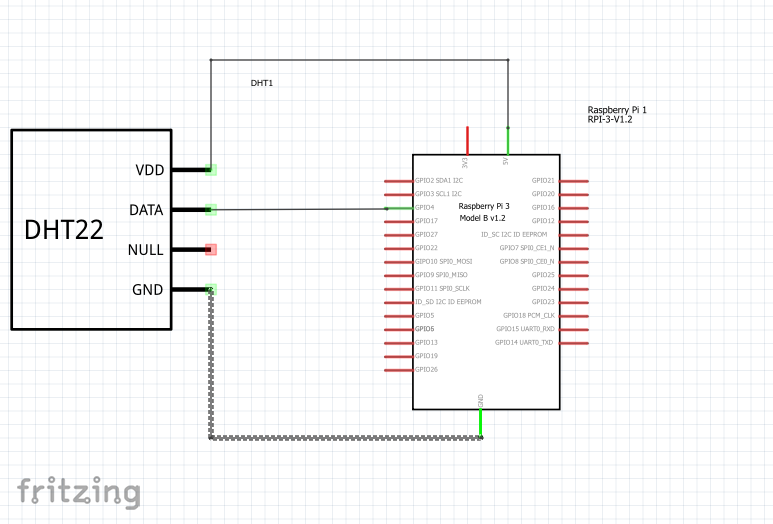
\includegraphics[width=\textwidth]{Images/schematicforDHT22.png}
		\caption{Schematic for DHT22}
		\label{Sychematic for DHT22 revised}
	\end{subfigure}
\end{figure}

From above the schematic is seen. DHT22 connections are the following:
\begin{itemize}
	\item VDD is connected to 5v of the Pi
	\item the Data pin is connected to GPIO 3
	\item Gnd pin  of the  Pi is  connected to the ground  of DHT22 

\end{itemize}
\cite{sparkfun} The following is the \href{https://www.sparkfun.com/datasheets/Sensors/Temperature/DHT22.pdf}{link} to the datasheet of this module
when reading from this  component. There is  a  delay  of 2 seconds due to the  sampling period.

\subsubsection{Light sensor}
In this section the following will be considered:
\begin{enumerate}
	\item What region the project is in 
	\item What light levels are expected in this  country
	\item What sensor  will  accommodate this  range
\end{enumerate}
\newpage
For this sensor  the outside aspect of the  project must also be considered.The following table was found on \cite{wiki_2023}:
	\begin{table}[h!]
	\centering
	\begin{tabular}{|l|l|}
	\hline
		Imminence & Example \\ \hline
		**0.002 lux** & Moonless clear night sky \\ \hline
		**0.2 lux** & Design minimum for emergency lighting (AS2293). \\ \hline
		**0.27 \& 1 lux** & Full moon on a clear night \\ \hline
		**3.4 lux** & Dark limit of civil twilight under a clear sky \\ \hline
		**50 lux** & Family living room \\ \hline
		**80 lux** & Hallway/toilet \\ \hline
		**100 lux** & Very dark overcast day \\ \hline
		**300 to 500 lux** & Sunrise or Sunset on a clear day. Well-lit office area. \\ \hline
		**1,000 lux** & Overcast day; typical TV studio lighting \\ \hline
		**10,000 to 25,000 lux** & Full daylight (not direct sun) \\ \hline
		**32,000 to 130,000 lux** & Direct sunlight \\ \hline
	\end{tabular}
	\caption{Illuminates values}
	\label{Illuminates values}
\end{table}
	This table is the  associated lux level  indicating when the values are . 
	From  above the sensor should ideally be 0.002 to 25000 lux, Bearing this in mind  these components were researched:
	\begin{table}[h!]
	\small
	\centering
	\begin{tabular}{|l|l|l|l|l|}
	\hline
		Modules & Voltage Range & Analogue /Digital Outputs & illumination range & Current rating \\ 
		\hline
		LM393 with GL5528 & 3.3v to 5v & Analogue & 0 lux to 100lux & 250nA \\ 
		\hline
		DFR0026 & 3.3v to 5v & Analogue & 1 Lux to 6000 Lux & 120uA \\ \hline
		LM393 with n5ac501085 & max 150V & Analogue & 10 lux to 100lux & 1mW \\ 
		\hline
		LM393 with NSL-06S53 & max 100v & analogue & 1 to 100 & 50mw \\ \hline
	\end{tabular}
	\caption{table of light sensors}
	\label{table of light sensors}
\end{table}
\newpage

After research DFR0026 \cite{DFR0026} is the option proposed for use as it is the best for this application,  which will have an analogue  output to see the interface (see below):

\begin{figure}[h!]
	\centering
	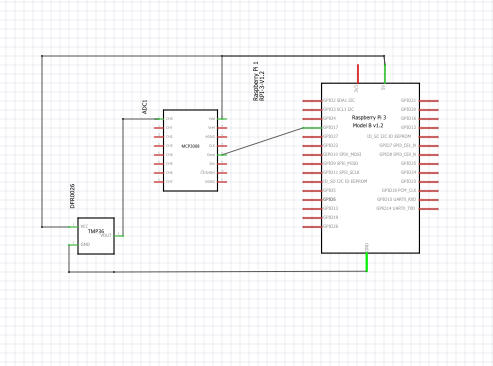
\includegraphics[width=0.6\linewidth]{Images/InterfaceofDFR0026.png}
	\caption{Interface for  DFR0026}
	\label{Interface for  DFR0026}
\end{figure}

The following are  the connections:
\begin{enumerate}
	\item VCC pin is connected  to 5v
	\item Gnd of the  sensor is connected to Gnd of the Pi
	\item The output is connected to  ch 0
	\item the output ranges  from  0 to  5 v
\end{enumerate}
The component relies on the  ADC  which  is on page\pageref{Adc section}

\subsubsection{Motion sensor}

For this section the following must be considered:
\begin{enumerate}
	\item The range of the  sensor
	\item The degree of the  sensor
	\item How long of a  delay is the sensor
\end{enumerate}
The  following are  the components considered:
\begin{table}[h!]
	\centering
	\begin{tabular}{|c|c|c|c|c|c|}
		\hline
		Modules & Voltage Range & Distance & Max angle & Analogue /Digital Outputs & Power \\
		\hline
		HC-SR501 & 5-20V & 3 to 7m & 110 & Digital & 50uA \\
		AM312 & 4.5-20v & 3m & 130 & Digital & 60uA \\
		AS312 & -0.3 - 3.6V & 12m & 130 & Digital & 100mA \\
		\hline
	\end{tabular}
	\caption{Motion sensor components}
	\label{Motion sensor components}
\end{table}

The sensor chosen is AS312\cite{micros}(which has a delay time of 2 seconds) which is a digital interface to see the wiring ,See below:
\newpage
The following is the interface for the device:

\begin{figure}[h!]
	\begin{center}
		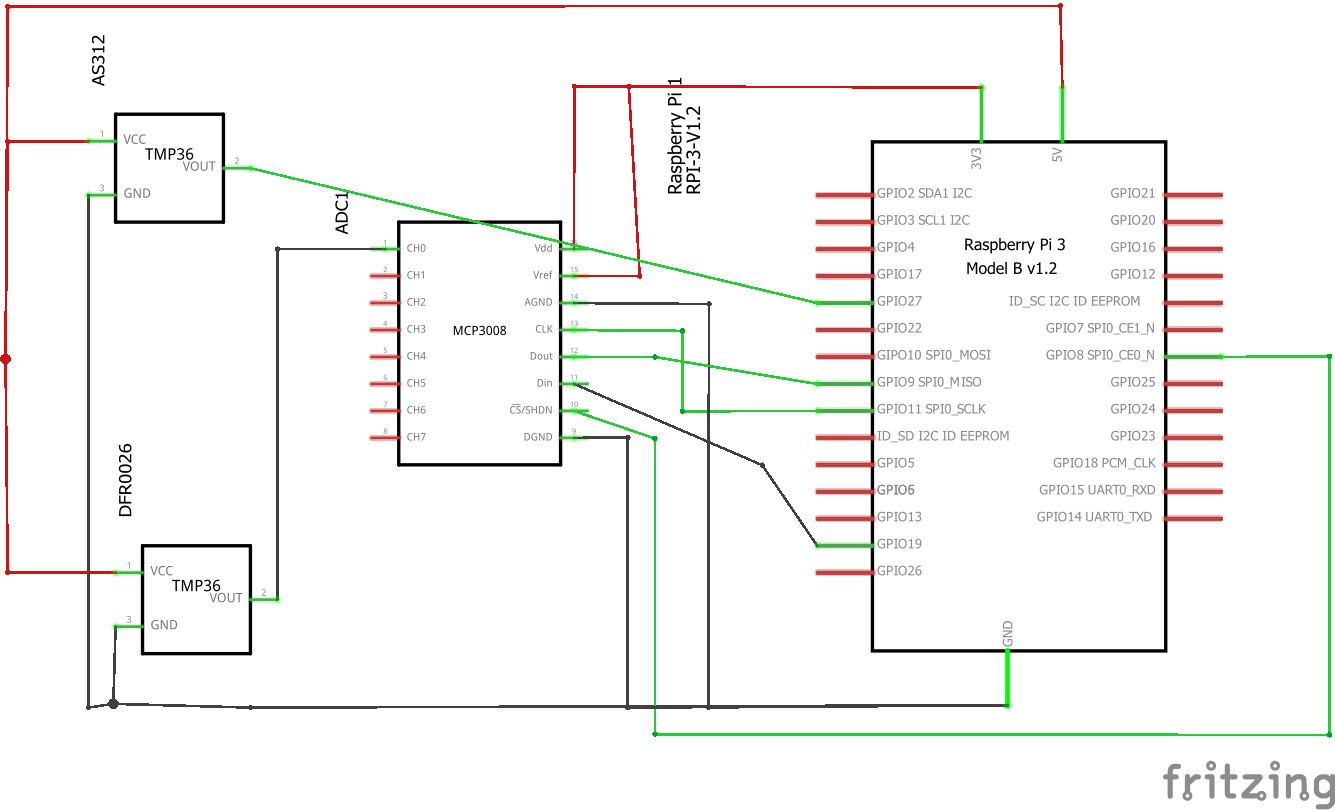
\includegraphics[width=0.5\linewidth]{Images/interfaceofAS312.png}
	\caption{Interface for AS312}
	\label{Interface for AS312}
	\end{center}

\end{figure}
The connections are the following:
\begin{figure}[h!]
	\centering
	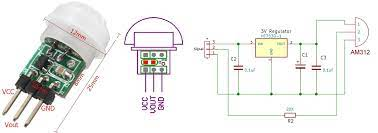
\includegraphics[width=0.5\linewidth]{Images/pinout_of_AS312.jpg}
	\caption*{Pinout of  AS312}
	\label{Pinout of  AS312}
\end{figure}
\begin{enumerate}
	\item VCC is connected  to 5v pin of the Pi
	\item GND is connected to the GND of the  Pi
	\item Vout is connected to GPIO 17
\end{enumerate}
This  component has the following:
\begin{enumerate}
	\item Range  of 12 meters 
	\item An  angle  of  65$^o$ degree
	\item A Delay of 15 $\mu$ Seconds
\end{enumerate}

\newpage
\subsection{Radio Module}
For this section there are the following considerations:
\begin{itemize}
	\item The devices are in a forest
	\item Meaning  Gigahertz  isn't  a desirable frequency
	\item A module that has low-power
	\item A model that  will have a high throughput 
\end{itemize}

Through research, I found the following table:
\begin{table}[h!]
	\centering
	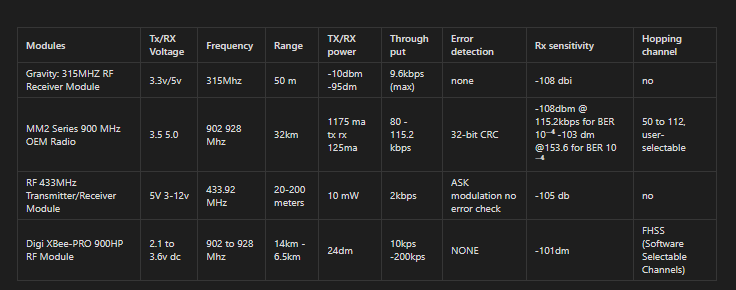
\includegraphics[width=0.5\linewidth]{Images/radiomoudles.png}
		
	\caption{Radio modules found in research}
	\label{Radio modules found in research}
	
\end{table}

Out of these, the MM2 Series 900 MHz\cite{freewave} was chosen.Note that the seller of this  radio module has  limited the documentation  of this module.This makes it hard to  draw an interface for this module .
\subsection{ADC Considerations}
\label{Adc section}
For the ADC  there are the following considerations:
\begin{enumerate}
	\item Low power
	\item High bit resolution
	\item Low number of channels
	\item High sample rate
\end{enumerate}
The two things needed for this is a high bit  Resolution  and  a  high sample rate
\begin{table}[h!]
	\begin{center}
		\begin{tabular}{|c|c|c|c|c|}
			\hline
			Device & Resolution & Sample rate & Input range & Power consumption \\
			\hline
			ADC pi Zero & 17 bits & 100KHz & 0-5.06v & 10mA \\
			MCP3008 & 10 bits & 200 ksps & 2.7v- 5.5v & 500uA \\
			DFR0553 & 16 bits & ~1.7Mhz & 0~5.0V&10mA\\
			\hline
		\end{tabular}
	\end{center}
\end{table}

Above are the components  to choose from 
for this project,MCP3008 was chosen due to its  resolution and  sample rate
\newpage
The following is the schematic for the  MCP3008\cite{ada}
\begin{figure}[h!]
	\centering
	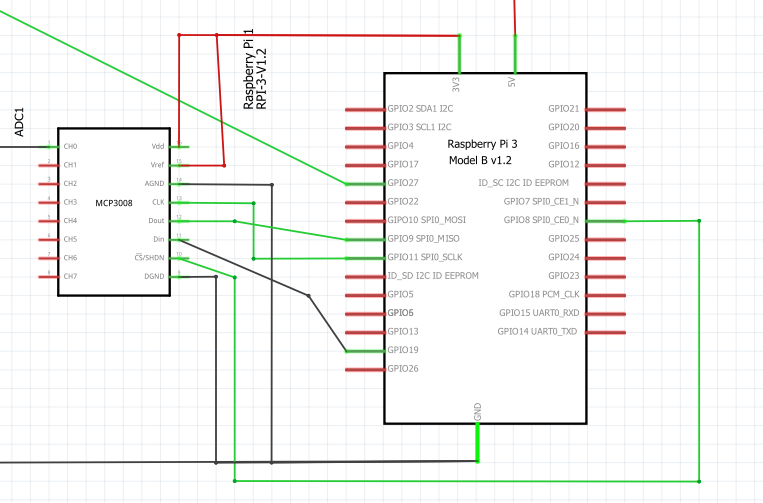
\includegraphics[width=0.6\linewidth]{Images/SchematicforMCP300.png}
	\caption{Schematic for  MCP3008}
	\label{Schematic for  MCP3008}
\end{figure}

The following are connections:
\begin{enumerate}
	\item VDD is connected to 3v3 pin of the  Pi
	\item VRef is  also connected to  3v3 pin of the  Pi
	\item AGND is connected to the gnd pin 
	\item CLK pin is connected to GPIO port 11
	\item Dout pin is connected to GPIO port 9
	\item Din pin is connected to GPIO port 19
	\item CS pin  is connected  to GPIO port 8
	\item DGND ping is connected to the gnd pin
\end{enumerate}

This  component has the following:
\begin{enumerate}
	\item A 10 bit resolution
	\item Seen as  the  reference  will  be 3.3v  
	\item 200ksps, meaning the delay to read is 5$\mu$ seconds
\end{enumerate}

\subsection{Camera}
For the camera,  the following has to be considered:
\begin{enumerate}
	\item Focal length
	\item Resolution
	\item Power
	\item The lux values it operates at
\end{enumerate}
\begin{table}[h!]
	\centering
	\scalebox{0.6}{\begin{tabular}{|c|c|c|c|c|c|c|c|c|}
	
		\hline
		Modules & Voltage range & lens size & Image Resolution & Video Resolution & Frame Rate & Type of Output & Preferred condition & Power \\
		Raspberry Pi VR 220 Camera & 3.3V ac &can change with lens & 3280 X 2462 & 1920 x 1080 &  30 FPS & Need to research & Daytime & 38mA \\
		DIGILENT 410-358 & 3.6v &  optical size 1/4 inches  & 2592 x 1944 &? &? &Digital &? & 200mA \\
		The Raspberry Pi NoIR & 3.3v  & 1/4 inches  &3280 x 2464  & 1080 or 720  &30 60 fps &need to research & house & 38mA \\
		OV7670 VGA & 2.45 to 3.0v ac & 1/6 inches & 2.36mm x 3.6um &? & 30 fps & analogue &  need to research &60mW \\
		\hline
	\end{tabular}}
	\caption{Camera module}
	\label{Camera module}
\end{table}

The camera chosen is a Raspberry Pi VR 220\cite{RS} Camera To see how to connect look at the  following \href{https://youtu.be/yhM1NhD-kGs?si=yxgFZb84yxSGLtM3}{link}. 
\subsection{Memory module}
For this section, we consider the following:
\begin{enumerate}
	\item The file formatting of the sensor data
	\item The file formatting of  the camera data
	\item What are  the possible sizes of data
	\item What is the  memory size of the  raspberry pi OS
\end{enumerate}

In my project the following is used:
\begin{enumerate}
	\item The sensor data  is stored in a  CSV file with the following heading: (timestamp, heat, humidity, light level, anything detected), Which can be around 25KB
	\item For the camera using 10 MB is the  largest file  size
	\item For the Raspberry Pi  downloaded  the raspberry imager , This has  lots of  options such as  the  following on page \pageref{pi os}
\end{enumerate}

After has been we must consider a  mircoSD ,The following are considerations:
\begin{table}[h!]
	\begin{tabular}{|c|c|c|c|c|c|c|c|c|c|}
		\hline \\
		Product Name & Capacity & Speed class & Read speed & Write speed & Temperature range & Operating volatage &Shock Resistance &Vibration Resistance \\
		\hline \hline
		SAMSUNG EVO Plus Class 10 microSDXC& 256 GB &U3&up to 130MB/s&up to 130MB/s&N/A&N/A&yes&yes \\
		SANDISK Ultra Performance Class 10 microSDXC&128 GB& class 10 u1&up to 80 MB/s&up to 10 MB/s&N/A&N/A&yes&yes \\
		Silicon Power 32GB 3D&32GB &class 10&Up to 100MB/s&Up to 100MB/s&0 to 70&2.7v - 3.6v&yes&yes \\
		SanDisk 64GB Extreme PRO&64GB&UHS Speed Class 3&Up to 100MB/s& up to 90 MB/s&N/A&N/A&yes&yes \\
		\hline
	\end{tabular}
	\caption{Mirco SDs in consideration}
	\label{mirco SDs in consirdation}
\end{table}

The best here is the silicon power 32GB due to its temperature range and read and write times.
we can consider extra memory: 
\begin{enumerate}
	\item DHTT22 has a sample period of  2 seconds
	\item AS312 which has a  delay time of 15 $\mu$ seconds
	\item MCP3008 5 $\mu$ seconds
\end{enumerate}

Through research,the following was discovered :
\begin{table}[h!]
	\centering
	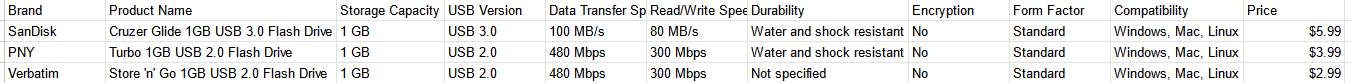
\includegraphics[width=0.8\linewidth]{Images/memory_devices.png}
	\caption{Memory usb to consider}
	\label{Memory usb to consider}
\end{table}

The Raspberry Pi 4 supports USB 2 and  USB 3. For this, the Turbo 1GB USB 2 Flash Drive will  be chosen.

\subsection{Battery}
In this section the  following must be considered:
\begin{enumerate}
	\item Enough power for all  sensors  and  radio module
	\item Storage of the battery
	\item Discharge rate of the  battery (how many operating hours can be got out of the  battery)
\end{enumerate}
Here are the following  Devices I found :
\begin{table}[h!]
	\centering
	\begin{tabular}{|c|c|c|c|c|c|}
		\hline
		Modules & Voltage & Interface & Power & Chemistry & Supply time\\
		\hline
			Li-polymer Battery HAT  & 5v & Micro USB & 1.8A &lithium battery &5 hours \\ \hline
	\end{tabular}
	\caption{battery considerations}
	\label{battery considerations}
\end{table}

The battery chosen  is the li-polymer which has a micro USB 
How to charge:
\begin{itemize}
	\item Step 1: Insert the Li-polymer battery into a 2.0mm battery socket
	\item Step 2: Connect the power adapter to a micro USB or Type-C interface by USB cable.
\end{itemize}

Aside: this component has the following:
\begin{enumerate}
	\item A battery that is 3.7v 3000$mAh$ 
	\item Output voltage of 5 volts
	\item an estimated Power supply time  of  5 hours
\end{enumerate}
\subsection{Arduino vs PI Consideration }
In this project, we will have to choose between what microprocessor we will use.There are 3 options:
\begin{enumerate}
	\item PCB (printed circuit board)
	where the circuit is deigned in a program like Fusion 360. The major issue is due to  the current state of  silicon chips which will slow down  the progress of the implementation stage
	\item Arduino 
	\item Raspberry Pi
\end{enumerate}

The advantages and disadvantages of the Arduino and  the Raspberry Pi are the following:
\begin{table}[h!]
	\centering
	\begin{tabular}{|c|c|}
		\hline
		Arduino & Pi \\
	
	\hline \hline
	Advantages & Advantages \\
	\hline \hline
	1. Arduino has a 10-bit ADC & 1. Pi can compile Python (easier to write ) \\

	\hline \hline
	Disadvantages & Disadvantages \\
	\hline \hline
	1. Arduino has a supper set of C++ & 1. Pi is a technically a small CPU \\
	2. Arduino only has 6 Analogue pins  & 2. The Pi needs an ADC circuit to deal with inputs that are analogue \\
	
	\hline
	\end{tabular}
	\caption{Advantages /Disadvantages of Arduino vs pi}
	\label{Advantages /Disadvantages of Arduino vs pi}
\end{table}

Although the  Arduino would be more efficient than the Raspberry Pi due to Raspberry Pi has an Operating System . The Pi was picked due familiar with Python and Linux. Linux can  be used to handle the networking side  of   the project
At the cost of  some efficiency in power for an easier time writing the code for  this  project 
\subsubsection{Picking a Raspberry Pi}
Now that a device was chosen to  use the following need to be defined:
\begin{enumerate}
	\item The amount of GIPO PORTS we need 
	\item Nature of the output of the sensor
	\item Speed of the clock
\end{enumerate}	

GPIO(General purpose input/output) is used  to select the input/output. The Pi can  take in  digital signals only Seen as the components are chosen that require A GPIO port (temperature/ humidity, on page \pageref{Compareing DHT22 and DHT11}, Light on page \pageref{table of light sensors}, motion on page \pageref{Motion sensor components})

At least  3 GPIO ports to be available to us as the light sensor and the motion will  need  an adc as looking through the documentation .firstly let's look at the  different models:
\begin{table}[h!]
\scalebox{0.6}{\begin{tabular}{|l|l|r|l|l|l|1|}
	\hline
	\rowcolor[HTML]{CE6301} 
	Raspberry Pi Model      & Internal Clock Speed & \multicolumn{1}{l|}{\cellcolor[HTML]{CE6301}Power (Watts)} & GPIO Features & Type of Connectors                                                            & SRAM                   \\ \hline
	Raspberry Pi 1 Model B+ & 700 MHz              & 5.5                                                        & 26 GPIO pins  & 1 HDMI, 1 micro USB, 1 USB 2.0, 1 audio jack                                   & 512 MB                 \\
	Raspberry Pi 2 Model B  & 900 MHz              & 7.5                                                        & 40 GPIO pins  & 1 HDMI, 1 micro USB, 4 USB 2.0, 1 audio jack                                   & 1 GB                   \\
	Raspberry Pi 3 Model B+ & 1.4 GHz              & 8                                                          & 40 GPIO pins  & 1 HDMI, 1 micro USB, 4 USB 2.0, 1 audio jack, 1 Gigabit Ethernet, 1 PoE header & 1 GB                   \\
	Raspberry Pi 3 Model A+ & 1.4 GHz              & 5                                                          & 26 GPIO pins  & 1 HDMI, 1 micro USB, 2 USB 2.0, 1 audio jack                                   & 512 MB                 \\
	Raspberry Pi Zero       & 1 GHz                & 1.2                                                        & 40 GPIO pins  & 1 mini HDMI, 1 micro USB, 1 micro-USB OTG                                      & 512 MB                 \\
	Raspberry Pi Zero W     & 1 GHz                & 1.3                                                        & 40 GPIO pins  & 1 mini HDMI, 1 micro USB, 1 micro-USB OTG, 1 Wi-Fi/Bluetooth module            & 512 MB                 \\
	Raspberry Pi Zero 2 W   & 1 GHz                & 0.8                                                        & 40 GPIO pins  & 1 mini HDMI, 1 micro USB, 1 micro-USB OTG, 1 Wi-Fi/Bluetooth module            & 512 MB                 \\
	Raspberry Pi 4 Model B  & 1.5 GHz              & 7                                                          & 40 GPIO pins  & 2 HDMI, 2 USB 3.0, 2 USB 2.0, 1 Gigabit Ethernet, 1 audio jack                & 1 GB, 2 GB, 4 GB, 8 GB \\ \hline
	\hline
\end{tabular}
}
\caption{Table of Raspberry Pi's}
\label{Table of Raspberry Pi's}
\end{table}

The above table displays the modules ,As our radio modules is 900Mhz  we want  1.5GHZ which is the Raspberry Pi 4.This needs a USB\- c charger and an HDMI mini cable.
For wiring our Pi here is  the GPIO pin layout:
\begin{figure}[h!]
	\centering
	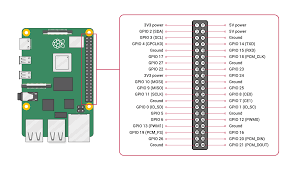
\includegraphics[width=0.8\linewidth]{Images/Pinout_of_pi.png}
	\caption*{Pinout for  the  pi}
	\label{Pinout for  the  pi}
\end{figure}

\subsection{Conclusion}
In this project the hardware needed is the  following components:
\begin{enumerate}
	\item 1 x Raspberry Pi 4 Model B 
	\item 1 x HDMI cable
	\item 1 x USB\-C cable
	\item 1 x USB \-C charging head
	\item 1 x DHT22
	\item 1 x DFR0026
	\item 1 x AS312
	\item 1 x MM2 Series 900 MHz
	\item 1 x MCP3008
	\item 1 x Raspberry Pi VR 220 Camera
	\item  1 x Li-polymer Battery HAT 
	\item 1 x Turbo 1GB
	\item 1 x silicon power 32GB  microSD
	
	
\end{enumerate}